% =============================================================
%  math-figure-svg — TikZ 方案示例
%  以 AB 为直径的半圆与几何平均（CD = sqrt(ab)）
%
%  核心思想：几何与数学「同源」。
%  图形（半圆、直径、垂线、直角标记、各点）和数学公式
%  （AB = a + b、AC = a、CB = b、CD = sqrt(ab)）来自同一份
%  LaTeX 源码，公式全部由 TeX 本身排版，永远不会「画歪」。
%
%  编译（见 build.sh）：
%    latex semicircle-mean.tex          ->  semicircle-mean.dvi
%    dvisvgm -n -o semicircle-mean.svg semicircle-mean.dvi
%  或用 pdflatex 出 PDF，再用 pdftocairo/pdf2svg/inkscape 转 SVG。
% =============================================================
\documentclass[tikz, border=6pt]{standalone}
\usepackage{tikz}
\usetikzlibrary{calc, angles, quotes}   % angles 用于直角标记
\usepackage{amsmath, amssymb}

\begin{document}
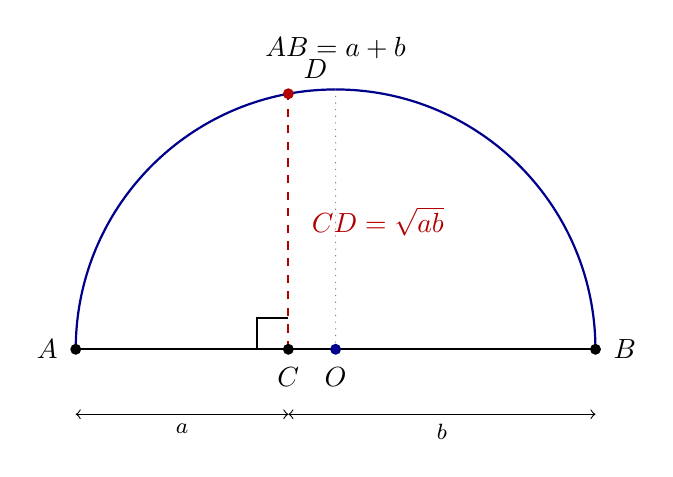
\begin{tikzpicture}[
    scale=1.5,
    dot/.style = {circle, fill, inner sep=1.4pt, outer sep=0pt},
    lbl/.style = {font=\footnotesize},
  ]

  % ---------- 参数：只改这里即可换图 ----------
  \def\a{1.8}                 % AC = a
  \def\b{2.6}                 % CB = b
  \pgfmathsetmacro{\AB}{\a+\b}        % AB = a + b
  \pgfmathsetmacro{\R}{\AB/2}         % 半径 = AO = OB（圆心 O）
  \pgfmathsetmacro{\h}{sqrt(\a*\b)}   % CD = sqrt(ab)，几何平均

  % ---------- 关键点 ----------
  \coordinate (A) at (0,0);
  \coordinate (B) at (\AB,0);
  \coordinate (C) at (\a,0);
  \coordinate (O) at (\R,0);
  \coordinate (D) at (\a,\h);

  % ---------- 半圆（直径 AB，圆心 O）----------
  \draw[thick, blue!55!black] (A) arc (180:0:\R);
  % ---------- 直径 AB ----------
  \draw[thick] (A) -- (B);

  % ---------- 过 C 的垂线，交半圆于 D ----------
  \draw[dashed, thick, red!70!black] (C) -- (D);

  % ---------- 直角标记（C 处，∠ACD）----------
  \draw pic[draw, thick, angle radius=4mm, angle eccentricity=1]
        {right angle = A--C--D};

  % ---------- 圆心 O 到弧顶的半径（虚线，强调圆心）----------
  \draw[dotted, thin, gray] (O) -- (\R,\R);

  % ---------- 端点 / 分点标注 ----------
  \node[dot]                 at (A) {}; \node[left=3pt]        at (A) {$A$};
  \node[dot]                 at (B) {}; \node[right=3pt]       at (B) {$B$};
  \node[dot]                 at (C) {}; \node[below=3pt]       at (C) {$C$};
  \node[dot, blue!55!black]  at (O) {}; \node[below=3pt]       at (O) {$O$};
  \node[dot, red!70!black]   at (D) {}; \node[above right=2pt] at (D) {$D$};

  % ---------- 上方的整体关系 ----------
  \node[above] at (\R, \R+0.18) {$AB = a + b$};

  % ---------- 下方的分段标注 a / b ----------
  \draw[<->, lbl] ([yshift=-0.55cm]A) -- ([yshift=-0.55cm]C)
        node[midway, below] {$a$};
  \draw[<->, lbl] ([yshift=-0.55cm]C) -- ([yshift=-0.55cm]B)
        node[midway, below] {$b$};

  % ---------- CD 的关系（几何平均）----------
  \node[right=5pt, red!70!black] at ($(C)!0.5!(D)$) {$CD = \sqrt{ab}$};

\end{tikzpicture}
\end{document}
